\section{Procesos}
\subsection{Introduccion}

Un proceso es una abstracción de un programa en ejecución, que básicamente convierte una CPU en varias CPU virtuales, proporcionando de esta manera la capacidad de operar (pseudo)concurrentemente, incluso cuando hay una sola CPU disponible.

Un proceso no es más que una instancia de un programa en ejecución, incluyendo los valores actuales del contador de programa, los registros y las variables. En concepto, cada proceso tiene su propia CPU virtual; en la realidad, la CPU real conmuta de un proceso a otro. Varios procesos pueden compartir un solo procesador mediante el uso de un algoritmo de planificación para determinar cuándo se debe detener el trabajo en un proceso para dar servicio a otro.

Hay cuatro eventos principales que provocan la creación de procesos:
\begin{itemize}
\item El arranque del sistema
\item La ejecución de una llamada al sistema para creación de procesos.
\item Una petición de usuario para crear un proceso.
\item El inicio de un trabajo por lotes.
\end{itemize}

Algunos procesos corren en primer plano, es decir, interactúan con los usuarios, mientras que otros procesos, que no están asociados con usuarios específicos sino con una función específica, corren en segundo plano. Un ejemplo sería un proceso que acepte peticiones entrantes para las páginas web hospedadas en ese equipo; estos procesos se conocen como \textbf{daemons}.

En UNIX sólo hay una llamada al sistema para crear un proceso: \textbf{fork}. Esta llamada crea un clon exacto del proceso que hizo la llamada. Después del fork, los dos procesos (padre e hijo) tienen la misma imagen de memoria, las mismas variables de entorno y los mismos archivos abiertos. Por lo general, el proceso hijo ejecuta después a \textbf{execve} o una llamada al sistema similar para cambiar su imagen de memoria y ejecutar un nuevo programa. La razón de este proceso de dos pasos es para permitir al hijo manipular sus descriptores de archivo después de fork, pero antes de execve, para poder lograr la redirección de la entrada, salida y error estándar.

\subsection{Estados de un proceso}

Un proceso se puede encontrar en uno de tres estados:

\begin{itemize}
\item En ejecución (está usando la CPU en ese instante)
\item Listo (ejecutable. Se detuvo temporalmente para dejar que se ejecute otro proceso.)
\item Bloqueado (no puede ejecutarse hasta que ocurra cierto evento externo)
\end{itemize}

~\\
\begin{figure}[h]
	\begin{center}
	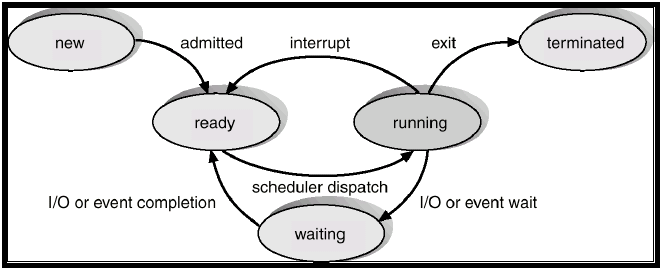
\includegraphics[width=0.8\textwidth]{imagenes/processstates.png}
	\caption{Estados de un proceso}
	\end{center}
\end{figure}
~\\

\subsection{Implementación de los procesos}

Para implementar el modelo de procesos, el SO mantiene una tabla llamada tabla de procesos, con una entrada por cada proceso (llamada Process Control Block (PCB)). Esta entrada contiene información importante acerca del estado de cada proceso, como el Program Counter, el Stack Pointer, asignación de memoria, estado de sus archivos abiertos, información para el scheduler, registros de la CPU, etc.

Cuando ocurre una interrupción, el PC, el PSW, y uno o más registros se meten en la pila mediante el hardware de interrupción. Después, la CPU salta a la dirección especificada en el vector de interrupción. Esto es todo lo que hace el hardware, en adelante es todo responsabilidad del software.

Todas las interrupciones comienzan por guardar los registros, a menudo en la entrada de la tabla de procesos para el proceso actual. Después, se quita la información que la interrupción metió en la pila y el stack pointer se establece para que apunte a una pila temporal utilizada por el manejador de procesos.

Cuando se terminan de guardar los registros, se llama a un procedimiento para realizar el resto del trabajo para este tipo de interrupción específica. Cuando termina su trabajo y tal vez algún otro proceso está listo, el scheduler es llamado para ver qué proceso se debe ejecutar a continuación. Después de eso, el control pasa de vuelta al código en lenguaje ensamblador para cargar los registros y el mapa de memoria para el proceso que entonces es el actual.

Un resumen de los pasos que ejecuta el sistema operativo cuando ocurre una interrupción es el siguiente:

\begin{enumerate}[1]
\item[1)] El hardware mete el PC, PSW, registros, etc. a la pila.
\item[2)] El hardware carga el nuevo PC del vector de interrupciones.
\item[3)] Procedimiento en lenguaje ensamblador guarda los registros.
\item[4)] Procedimiento en lenguaje ensamblador establece la nueva pila.
\item[5)] El servicio de interrupciones de C se ejecuta.
\item[6)] El scheduler decide qué proceso se va a ejecutar a continuación.
\item[7)] Procedimiento en C regresa al código en ensamblador.
\item[8)] Procedimiento en lenguaje ensamblador inicia el nuevo proceso actual.
\end{enumerate}

A continuación un ejemplo de una interrupción en el contexto de una syscall:

~\\
\begin{figure}[h]
	\begin{center}
	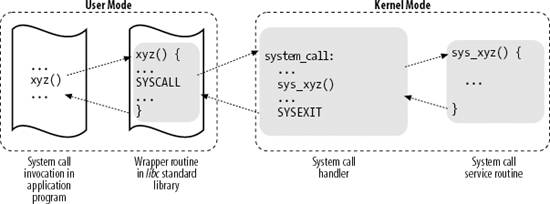
\includegraphics[width=0.8\textwidth]{imagenes/syscall.png}
	\caption{syscall}
	\end{center}
\end{figure}
~\\

\subsection{Threads}

Los threads son una especie de "mini roceso" o "proceso ligero" dentro de un proceso clásico. Los threads posibilitan el concepto de procesos secuenciales que realizan llamadas al sistema con bloqueo y de todas formas logran paralelismo.

Una manera de ver a un proceso es como si fuera una forma de agrupar recursos relacionados, como archivos abiertos, procesos hijos, etc., además de su espacio de direcciones. El otro concepto que tiene un proceso es el de hilo de ejecución, el cual tiene un contador de programa, registros con sus variables actuales y una pila. Aunque un hilo se deba ejecutar en cierto proceso, el hilo y su proceso son conceptos distintos y pueden tratarse por separado.

Lo que agregan los hilos al modelo de procesos es permitir que se lleven a cabo varias ejecuciones en el mismo entorno del proceso, que son en gram parte independientes, por lo tanto, los hilos dentro de un proceso comparten el mismo espacio de direcciones. No hay protección entre los hilos debido a que (1) es imposible y (2) no debe ser necesario. A diferencia de tener procesos diferentes, que pueden ser de distintos usuarios y hostiles entre sí, un proceso siempre es propiedad de un solo usuario, quien se supone ha creado varios hilos para que cooperen. Además de compartir un espacio de direcciones, todos los threads pueden compartir el mismo conjunto de archivos abiertos, procesos hijos, señales, etc. Al igual que un proceso tradicional, un thread puede estar en uno de varios estados: ene ejecución, bloqueado, listo o terminado.

Hay 2 formas principales de implementar una librería de threads: en espacio de usuario o en el kernel, aunque también es posible una implementación híbrida.

\subsubsection{Implementación de threads en espacio de usuario}

En este caso la librería de threads reside completamente en espacio de usuario, y el kernel no sabe nada de ellos. En lo que al kernel concierne, está administrando procesos ordinarios con un solo thread.

En este caso, cada proceso tiene su propia tabla de threads. Algunas ventajas son que cuando un thread se bloquea y se debe conmutar con otro, el procedimiento es mucho más rápido que hacer el trap al kernel. Otra ventaja es que cada proceso puede tener su propio algoritmo de planificación personalizado.

A pesar de su buen rendimiento, los threads a nivel de usuario tienen algunos problemas importantes. El primero de todos es la manera en que se implementan las llamadas al sistema de bloqueo. Si, por ejemplo, un thread lee del teclado antes de que se haya oprimido una sola tecla, es inaceptable permitir que el thread se bloquée, ya que esto también bloqueará a todos los threads del proceso. Si un thread produce un fallo de página, el kernel naturalmente bloquea a todo el proceso, llevando al mismo problema que en el caso anterior.

Otro problema es que si un thread comienza a ejecutarse, ningún otro thread en ese proceso se ejecutará a menos que el primero renuncie de manera voluntaria a la CPU, ya que dentro de un proceso no hay interrupciones.

\subsubsection{Implementación de threads en el kernel}

En este caso, en vez de tener una tabla de threads por proceso, el kernel tiene una tabla de threads que lleva la cuenta de todos los threads del sistema. Además, el kernel mantiene la tabla de procesos tradicional. Cuando un proceso desea crear un nuevo thread, realiza una llamada al kernel. Los threads del kernel no requieren de nuevas llamadas al sistema no bloqueantes, y si se produce un fallo de página, el kernel puede comprobar con facilidad si el proceso tiene otros threads que puedan ejecutarse y los ejecuta. Su principal desventaja es que el costo de una llamada al sistema es considerable. Sin embargo, hay algunos problemas que no resuelven, como qué hacer luego de un fork, o qué hilo debe hacerse cargo de una señal enviada al proceso.

\subsubsection{Implementaciones híbridas}

Una manera de combinar los métodos anteriores es utilizar threads de nivel kernel y después multiplexar los threads de nivel usuario con alguno o todos los threads de nivel kernel. El programador puede determinar cuántos hilos de kernel va a utilizar y cuántos threads de nivel usuario va a multiplexar en cada uno.


\subsection{Sincronización entre procesos}

Los bugs que surgen cuando dos o más procesos están leyendo o escribiendo en algún buffer compartido y el resultado final depende de quién se ejecuta y exactamente cuándo lo hace, se conocen como \textbf{condiciones de carrera.}

Para evitar esto, se necesita \textbf{exclusión mutua}, es decir, cierta forma de asegurar que si un proceso está utilizando una variable o archivo compartido, los demás procesos se excluirán de hacer lo mismo. La parte del programa en la que se accede a la memoria compartida se conoce como \textbf{región crítica.}

Para solucionar esto, se busca cumplir las siguientes cuatro condiciones:

\begin{itemize}
\item No puede haber dos procesos de manera simultánea dentro de sus regiones críticas.
\item No pueden hacerse suposiciones acerca de las velocidades o el número de CPUs.
\item Ningún proceso que se ejecute fuera de su región crítica puede bloquear otros procesos.
\item Ningún proceso tiene que esperar para siempre para entrar a su región crítica.
\end{itemize}

Algunas proposiciones para lograr exclusión mutua son las siguientes:

\begin{itemize}
\item \textbf{\underline{Deshabilitar interrupciones:}} en un sistema con un solo procesador, la solución más simple es hacer que cada proceso deshabilite todas las interrupciones justo después de entrar a su región crítica y las rehabilite justo después de salir. A pesar de que esto soluciona el problema de las condiciones de carrera, introduce un nuevo problema, ya que si el proceso no rehabilita las interrupciones, el sistema no podría continuar ejecutándose.

En un procesador multinúcleo, al deshabilitar las interrupciones de una CPU no se evita que las demás CPUs interfieran con las operaciones que la primera CPU está realizando. En consecuencia, se requieren esquemas más sofisticados.

\item \textbf{\underline{Variables candado:}} es una solución por software que consiste en tener una variable compartida que está en 0 cuando no hay ningún proceso en su región crítica y 1 cuando si lo hay. Este método tiene el mismo problema que el anterior, ya que si 2 procesos leen el 0 a la vez, ambos fijarán el candado en 1 y entrarán en su región crítica.

\item \textbf{\underline{Alternancia estricta:}}
~\\
\begin{figure}[h]
	\begin{center}
	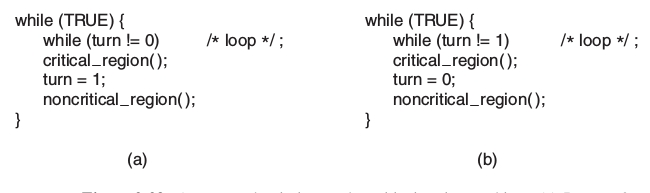
\includegraphics[width=0.8\textwidth]{imagenes/alternancia-estricta.jpg}
	\end{center}
\end{figure}
~\\

Cuando un proceso está evaluando continuamente una variable (como \textit{turn}), se dice que está haciendo \textbf{busy waiting}.

El problema con este enfoque es que si uno de los procesos es mucho más lento que el otro, este otro proceso quedará haciendo busy waiting hasta que el proceso más lento vuelva a cambiar la variable candado. Esta situación viola la condición 3 antes establecida: un proceso está siendo bloqueado por otro proceso que no está en su región crítica. Por más que evite las condiciones de carrera, no es un candidato serio como solución.
~\\

\item \textbf{\underline{Solución de Peterson:}}

\begin{figure}[h]
	\begin{center}
	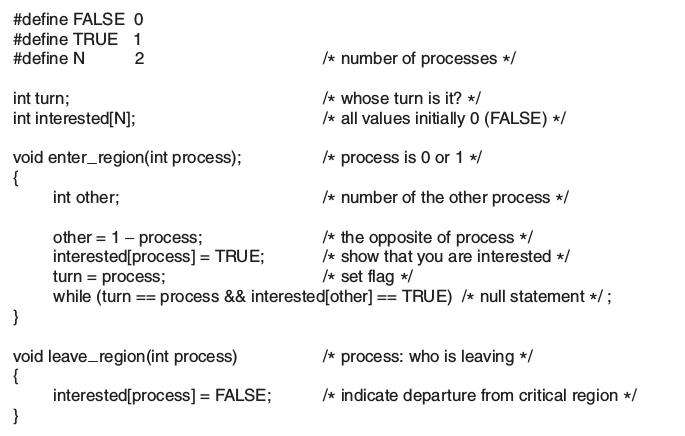
\includegraphics[width=0.8\textwidth]{imagenes/peterson.jpg}
	\end{center}
\end{figure}

\item \textbf{\underline{Instrucción TSL:}} TSL (test-and-set-lock) es una instrucción del hardware que funciona de la siguiente manera: lee el contenido de una palabra de memoria (candado) y lo guarda en un registro, y después almacena un valor distinto de cero en la dirección de memoria del candado. Se garantiza que las operaciones de leer la palabra y almacenar un valor en ella serán indivisibles; la CPU que ejecuta la instrucción TSL bloquea el bus de memoria para impedir que otras CPUs accedan a la memoria hasta que termine. Para lograr esto, se deshabilita el bus de memoria para el resto de los procesadores. Para usar la instrucción TSL necesitamos una variable compartida (candado) que coordine el acceso a la memoria compartida. Cuando candado es 0, cualquier proceso lo puede fijar en 1 mediante el uso de la instrucción TSL y después una lectura o escritura en la memoria compartida. Cuando termina, el proceso establece candado en 0 mediante una instrucción move ordinaria.

\item \textbf{\underline{sleep y wakeup:}} tanto la solución de Peterson como la solución mediante TSL son correctas, pero todas tienen el defecto de requerir busy waiting. Esto no solo desperdicia tiempo de CPU, sino que también puede tener efectos inesperados, por ejemplo, si hay 2 procesos H y L con prioridad alta y baja respectivamente, y H se ejecuta cada vez que se encuentra en el estado listo. En cierto momento, con L en su región crítica, H cambia al estado listo para ejecutarse y empieza a hacer busy waiting, pero como L nunca se planifica mientras H está en ejecución, L no puede salir de su región crítica y H queda iterando indefinidamente. A esta situación se la conoce como el problema de \textbf{inversión de prioridades}.

Una alternativa es usar ciertas primitivas para bloquear a los procesos que no pueden entrar a sus regiones críticas. Una de las más simples es el par \textbf{sleep} y \textbf{wakeup}. Como ejemplo de la forma en que se pueden usar, consideremos el problema del \textbf{productor-consumidor}: dos procesos comparten un buffer común de tamaño fijo. Uno de ellos (el productor) coloca datos en el buffer y el otro (el consumidor) los saca (esto se puede generalizar al caso de $m$ productores y $n$ consumidores).

El problema surge cuando el productor desea colocar un nuevo elemento en el buffer, pero este ya se encuentra lleno. La solución es que el productor se vaya a dormir y que se despierte cuando el consumidor haya quitado uno o más elementos, y de manera similar el consumidor se duerme si el buffer se encuentra vacío. Para llevar la cuenta del número de elementos en el buffer, necesitamos una variable (cuenta). Este método sin embargo produce condiciones de carrera, debido a que el acceso a cuenta no está restringido. Es posible que ocurra la siguiente situación: el buffer está vacío y el consumidor acaba de leer cuenta para ver si es $0$. En ese instante, el scheduler detiene al consumidor y empieza a ejecutarse el productor, el cual inserta un elemento en el buffer e incrementa cuenta, que ahora es $1$. Razonando que cuenta era antes $0$, y que por ende el consumidor debe estar dormido, el productor llama a wakeup para despertar al consumidor.

Como el consumidor todavía no estaba dormido, la señal se pierde. Cuando se vuelve a ejecutar el consumidor, evalúa el valor de cuenta que leyó antes, ve que es $0$ y pasa a dormirse. En algún momento el productor llena el buffer y se duerme. Ambos quedan dormidos para siempre.

El problema es que se envía una señal que se pierde. Una solución rápida es agregar un bit de espera, aunque esto también deja de funcionar con 3 o más procesos.

\item \textbf{\underline{Semáforos:}} un semáforo es una variable entera para contar el número de señales de despertar, almacenadas para un uso futuro. Cuenta con las funciones \textbf{down} y \textbf{up} (generalizaciones de sleep y wakeup). La función down comprueba si el valor es mayor que $0$. De ser así, disminuye el valor y sólo continúa. Si el valor es $0$, el proceso se pone a dormir sin completar la operación down por el momento. Las acciones de comprobar el valor, modificarlo y posiblemente pasar a dormir, se realizan como una sola acción atómica indivisible. Esta atomicidad es esencial para resolver problemas de sincronización y evitar condiciones de carrera.

La operación \textbf{up} incrementa el valor del semáforo. Si uno o más procesos estaban inactivos en ese semáforo, el sistema selecciona uno de ellos al \textbf{azar} y permite que complete su operación down. Por lo tanto, después de un up en un semáforo que contenga procesos dormidos, el semáforo seguirá en $0$ pero habrá un proceso dormido menos en él. La operación up también es indivisible.

En el caso del productor-consumidor, se utilizan 2 tipos de semáforos: uno es el \textbf{mutex}, que se utiliza para la exclusión mutua. Está diseñado para que un solo proceso pueda leer o escribir el buffer y sus variables asociadas en un momento dado.

El otro uso de los semáforos es para la sincronización, por ejemplo, para que el productor deje de ejecutarse cuando el buffer esté lleno, y que el consumidor deje de ejecutarse cuando esté vacío.


\item \textbf{\underline{Monitores:}} un monitor es una colección de procedimientos, variables y estructuras de datos que se agrupan en un tipo especial de módulo o paquete. Tienen una importante propiedad que los hace útiles para lograr la exclusión mutua: sólo puede haber un proceso activo en un monitor en un instante dado. Los monitores son una construcción del lenguaje de programación, por lo que el compilador sabe que son especiales y puede manejar las llamadas a las funciones del monitor en forma distinta a las llamadas a otras funciones. Es responsabilidad del compilador implementar la exclusión mutua en las entradas del monitor.

Aunque los monitores proporcionan una manera fácil de lograr la exclusión mutua, se necesita también una forma en la que los procesos se bloqueen cuando no puedan continuar. La solución está en la introducción de las \textbf{variables de condición}, junto con 2 operaciones asociadas: \textbf{wait} y \textbf{signal}. Cuando un procedimiento de monitor no puede continuar, realiza un wait en alguna variable de condición, lo cual hace que el proceso se bloquee. Un proceso, por ejemplo, el consumidor, puede despertar a su socio dormido mediante un signal en la variable de condición. Para evitar tener 2 procesos activos en el monitor al mismo tiempo, necesitamos una regla que indique lo que ocurre después de una operación signal. Hoare propuso dejar que el proceso recién despertado se ejecutara, suspendiendo el otro. Hansen propuso requerir que un proceso que realice una operación signal deba salir del monitor de inmediato.
\end{itemize}

\newpage


\section{Scheduling}

En un sistema con multiprogramación, con frecuencia se tienen varios procesos o hilos que comparten la CPU al mismo tiempo. Si solo hay una CPU disponible, hay que decidir cuál proceso se va a ejecutar a continuación. La parte del sistema operativo que realiza esa decisión se llama \textbf{scheduler} y el algoritmo que utiliza se conoce como \textbf{algoritmo de planificación}.

Casi todos los procesos alternan ráfagas de cálculos con peticiones de E/S (de disco). Por lo general la CPU opera durante cierto tiempo sin detenerse, y después se realiza una llamada al sistema para leer o escribir datos en un archivo. Cuando se completa la llamada al sistema, la CPU realiza cálculos de nuevo y así sucesivamente. A los procesos que invierten la mayor parte de su tiempo realizando cálculos se los llama limitados a cálculos, mientras que a los que están la mayor parte del tiempo esperando la E/S se los llama limitados a E/S (I/O-bound). A medida que las CPUs se vuelven más rápidas, los procesos tienden a ser más limitados a E/S, por lo tanto estos procesos deben obtener rápidamente la oportunidad de ejecutarse para emitir su petición de disco y mantenerlo ocupado.

Los algoritmos de planificación se pueden dividir en dos categorías según cómo manejan las interrupciones de reloj: un algoritmo \textbf{no apropiativo} (nonpreemptive) selecciona un proceso para ejecutarlo y después sólo deja que se ejecute hasta que el mismo se bloquea o hasta que libere la CPU en forma voluntaria. No se toman decisiones de planificación durante las interrupciones de reloj. Una vez que se haya completado el procesamiento de la interrupción de reloj, se reanuda la ejecución del proceso que estaba antes de la interrupción, a menos que un proceso de mayor prioridad esté listo para correr.

Por el contrario, un algoritmo de planificación \textbf{apropiativo} (preemptive) selecciona un proceso y deja que se ejecute por un máximo de tiempo fijo. Si sigue en ejecución al final del intervalo de tiempo, se suspende y el scheduler selecciona otro proceso para ejecutarlo. Para llevar a cabo la planificación apropiativa, es necesario que ocurra una interrupción de reloj al final del intervalo para que la CPU regrese el control al scheduler.

\subsection{Categorías de los algoritmos de planificación}

\begin{itemize}

\item \textbf{\underline{Procesamiento por lotes:}} en los sistemas de procesamiento por lotes no hay usuarios que esperen una respuesta rápida a una petición corta. En consecuencia, son aceptables los algoritmos no apropiativos, ya que reducen la conmutación de procesos y por ende mejora el rendimiento.

\item \textbf{\underline{Interactivos:}} en este caso la apropiación es esencial para evitar que un proceso acapare la CPU y niegue el servicio a los demás.

\item \textbf{\underline{De tiempo real:}} en los sistemas de tiempo real, aunque parezca extraño, la apropiación a veces no es necesaria debido a que los procesos saben que no se pueden ejecutar durante períodos extensos. La diferencia con los sistemas interactivos es que los sistemas de tiempo real sólo ejecutan programas destinados para ampliar la aplicación en cuestión.

\end{itemize}

Algunas metas de los algoritmos de planificación que aplican a todos los sistemas son:

\begin{itemize}
\item Equidad: otorgar a cada proceso una parte justa de la CPU.
\item Aplicación de políticas: verificar que se lleven a cabo las políticas establecidas.
\item Balance: mantener ocupadas todas las partes del sistema.
\end{itemize}

En los sistemas de procesamiento por lotes se utilizan tres métricas para verificar el desempeño de los sistemas: rendimiento, tiempo de retorno y utilización de la CPU. El \textbf{rendimiento (throughput)} es el número de trabajos por hora que completa el sistema. El \textbf{tiempo de retorno} es el tiempo estadísticamente promedio desde el momento en que se envía un trabajo por lotes, hasta el momento en que se completa. Es el tiempo de respuesta que tiene el usuario.

Un algoritmo que maximiza el rendimiento no necesariamente minimiza el tiempo de retorno. Por ejemplo, dada una mezcla de trabajos cortos y largos, un scheduler que siempre ha ejecutado trabajos cortos y nunca uno largo puede tener un rendimiento excelente pero a expensas de un terrible tiempo de retorno para trabajos largos.

Para los sistemas interactivos se aplican distintas métricas. La más importante es minimizar el \textbf{tiempo de respuesta}, es decir, el tiempo que transcurre entre emitir un comando y obtener el resultado.

Los sistemas de tiempo real tienen diferentes metas de planificación. Se caracterizan por tener tiempos límite que deben cumplir. Por ejemplo, si una computadora está controlando un dispositivo que produce datos a un paso regular, al no ejecutar el proceso de recolección de datos a tiempo se podría perder información.

\subsection{Planificación en sistemas de procesamiento por lotes}

\subsubsection{First-Come, First-Served (FCFS)}

Con este algoritmo, la CPU se asigna a los procesos en el orden en el que la solicitan. Es un algoritmo no apropiativo, por lo tanto los procesos no se interrumpen por haberse ejecutado demasiado tiempo. Si el proceso en ejecución se bloquea, el primer proceso en la cola se ejecuta a continuación. Cuando un proceso bloqueado pasa al estado listo, al igual que un trabajo recién llegado, se coloca al final de la cola. Tiene como ventaja que es sencillo de implementar.

\subsubsection{Shortest Job First (SJF)}

Es un algoritmo de procesamiento por lotes no apropiativo, que asume que los tiempos de ejecución se conocen de antemano. Está orientado a maximizar el throughput. Sólo es óptimo cuando todos los trabajos están disponibles al mismo tiempo.

\subsubsection{Shortest Remaining Time Next (SRTN)}

Es una versión apropiativa de SJF.


\subsection{Planificación en sistemas interactivos}

\subsubsection{Round Robin}

A cada proceso se le asigna un intervalo de tiempo, conocido como \textbf{quantum}, durante el cual se le permite ejecutarse. Si el proceso se sigue ejecutando al final del quantum, la CPU es apropiada para dársela a otro proceso. Si el proceso se bloquea o termina antes de que haya transcurrido el quantum, la conmutación se realiza en ese momento.

La única cuestión interesante relacionada con este algoritmo es la longitud del quantum. Si se establece un quantum demasiado corto se producen demasiadas conmutaciones de procesos y se reduce la eficiencia de la CPU, pero si es demasiado largo se puede producir una mala respuesta a las peticiones interactivas cortas.

\subsubsection{Planificación por prioridad}

Round Robin hace la suposición implícita de que todos los procesos tienen igual importancia. La idea básica es: a cada proceso se le asigna una prioridad y el proceso ejecutable con la prioridad más alta es el que se puede ejecutar.

Para evitar que los procesos con alta prioridad se ejecuten de manera indefinida, el scheduler puede reducir la prioridad del proceso actual en cada pulso del reloj. De manera alternativa, a cada proceso se le puede asignar un quantum de tiempo máximo que tiene permitido ejecutarse.

Las prioridades se pueden asignar de manera estática o dinámica. Un ejemplo de esto último sería cuando algunos procesos que están muy limitados por la E/S requieren la CPU. En ese caso, el proceso debe recibir la CPU de inmediato para dejar que inicie su siguiente petición de E/S.

\subsubsection{Múltiples colas}

Se utilizan varias colas que representan distintas clases de prioridas. Por ejemplo, los procesos en la clase más alta se ejecutan durante un quantum, los de la siguiente clase durante 2 quantums, etc. Cada vez que un proceso utiliza todos los quantums que tenía asignados, se mueve una clase hacia abajo en la jerarquía.

\newpage

\section{Administración de memoria}

La parte del sistema operativo
